\documentclass[12pt]{article}
\usepackage[a4paper,margin=1in]{geometry}
\usepackage{listings}
\usepackage{xcolor}
\usepackage{graphicx}
\usepackage{hyperref}
\usepackage{titlesec}
\usepackage{setspace}
\usepackage{float} % For positioning figures
\onehalfspacing

\definecolor{codebg}{rgb}{0.95,0.95,0.95}
\lstset{
    backgroundcolor=\color{codebg},
    basicstyle=\ttfamily\footnotesize,
    breaklines=true,
    frame=single,
    captionpos=b,
    keywordstyle=\color{blue},
    commentstyle=\color{gray},
    stringstyle=\color{red},
    showstringspaces=false,
    language=C++
}

\titleformat{\section}{\large\bfseries}{\thesection}{1em}{}
\titleformat{\subsection}{\normalsize\bfseries}{\thesubsection}{1em}{}

\title{\textbf{Exploring Design Patterns: Facade and Flyweight}}
\author{Eazdan Mostafa Rafin \\
Roll Number: 2003055}
\date{\today}

\begin{document}

\maketitle

\section{Introduction}
In the world of software development, design patterns act like best practices or blueprints that guide developers to solve common problems in a structured way. Among the many patterns available, two particularly useful ones—especially in terms of simplifying code and improving performance—are the \textbf{Facade Pattern} and the \textbf{Flyweight Pattern}.

This report dives into these two patterns with real-life analogies, C++ implementations, and explanations designed to not only inform, but also make the concepts intuitive and approachable.

\section{Pattern 1: Facade}

\subsection{What is the Facade Pattern?}
The \textbf{Facade Pattern} provides a simplified interface to a complex subsystem. It allows clients to interact with multiple classes in a system through a single, unified interface — effectively hiding the complexity of the underlying implementation.

\subsection{Real-Life Analogy}
\subsubsection*{Smart Home System:}

Imagine living in a smart home. Before leaving the house, we usually do several things:
\begin{itemize}
    \item Turn off all the lights
    \item Set the thermostat to an energy-saving temperature
    \item Lock the doors and activate the security system
    \item Turn off the music
\end{itemize}

Doing all of this manually can be time-consuming and involves interacting with several different systems, each with its own interface.

Now, imagine your smart home app has a single \textbf{``Leave Home''} button. When you press it, all these tasks are performed automatically in the background.

This single button acts as a \textbf{facade} --- it provides a simplified interface to control multiple complex subsystems. 

\vspace{1em}

\noindent\textbf{Key Idea:} The \textit{Facade Design Pattern} is like that one button — it hides the complexity of multiple systems and provides an easy-to-use, unified interface.

\subsection{Visual Example}
A consumer calls one number and speaks with a customer service representative. The customer service representative acts as a Facade, providing an interface to the order fulfillment department, the billing department, and the shipping department.
\begin{figure}[H]
    \centering
    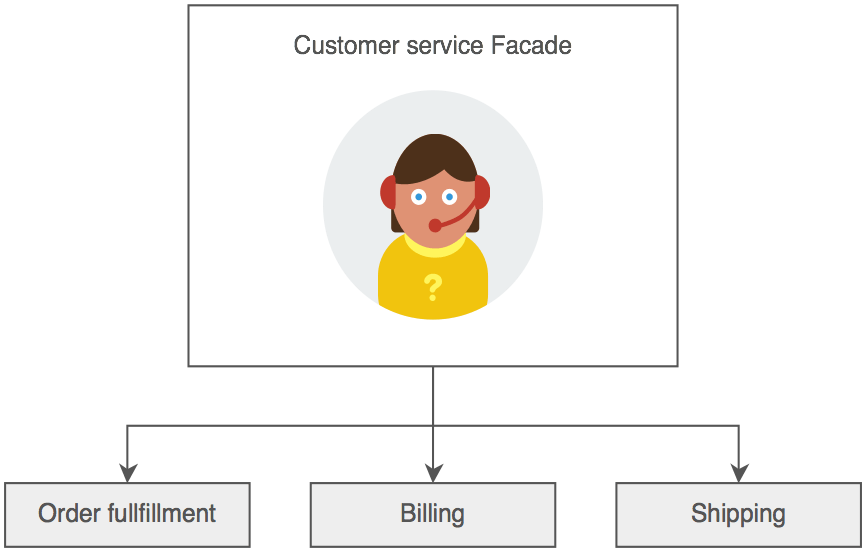
\includegraphics[width=\linewidth]{images/Facade_example.png} % Replace with your image file name
    \caption{Facade}
    \label{fig:sample_image}
\end{figure}



\subsection{C++ Example: Home Theater System}
\begin{lstlisting}[caption=Facade Pattern in a Home Theater System (C++)]
#include <iostream>
using namespace std;

class DVDPlayer {
public:
    void on() {
        cout << "DVD Player is now ON" << endl;
    }
    void play() {
        cout << "Playing the DVD..." << endl;
    }
};
class Projector {
public:
    void on() {
        cout << "Projector is warming up..." << endl;
    }
};
class SoundSystem {
public:
    void on() {
        cout << "Sound system is set to cinema mode" << endl;
    }
};
class HomeTheaterFacade {
private:
    DVDPlayer dvd;
    Projector projector;
    SoundSystem sound;
public:
    void watchMovie() {
        cout << "Initializing home theater setup..." << endl;
        dvd.on();
        projector.on();
        sound.on();
        dvd.play();
    }
};

// Main
int main() {
    HomeTheaterFacade homeTheater;
    homeTheater.watchMovie();
    return 0;
}
\end{lstlisting}

\section{Pattern 2: Flyweight}

\subsection{What is the Flyweight Pattern?}
The \textbf{Flyweight Pattern} is used to reduce memory consumption when working with a large number of similar objects. It separates the intrinsic (shared) state from the extrinsic (unique) state and reuses objects that share the same intrinsic data.

\subsection{Real-Life Analogy}
\subsubsection*{Text Editor Characters:}

Imagine we're using a text editor like Microsoft Word or Google Docs. As we type a long document, we end up with thousands of characters—letters, numbers, and symbols.

Each character may have formatting such as:
\begin{itemize}
    \item Font family (e.g., Arial, Times New Roman)
    \item Font size
    \item Style (bold, italic)
    \item Color
\end{itemize}

Storing every single character with all of its formatting would consume a large amount of memory, especially in longer documents.

To solve this, the text editor uses the \textbf{Flyweight Design Pattern}.

\vspace{1em}

\noindent\textbf{How it works:}
\begin{itemize}
    \item A shared object is created for each unique character format.
    \item The system reuses this shared object every time that specific style is needed.
    \item Only the unique information (like the character's position in the document) is stored separately.
\end{itemize}

For instance, if we have 5{,}000 occurrences of the letter ``e'' in the same font and style, the system only keeps one shared object instead of 5{,}000.

\vspace{1em}

\noindent\textbf{Key Idea:} The Flyweight Pattern allows us to efficiently manage memory by sharing common data across many objects, while keeping only the unique details separate.


\subsection{Visual Example}
When browser loads a web page, it traverse through all images on that page. Browser loads all new images from Internet and places them the internal cache. For already loaded images, a flyweight object is created, which has some unique data like position within the page, but everything else is referenced to the cached one.

\begin{figure}[H]
    \centering
    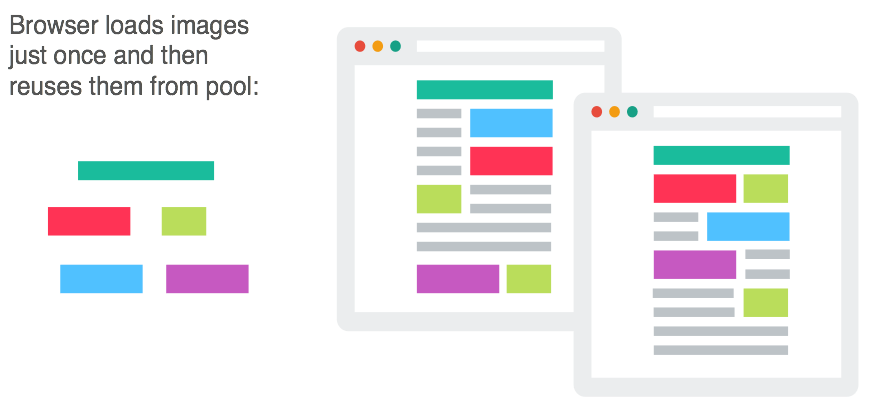
\includegraphics[width=\linewidth]{images/Flyweight_main.png} % Replace with your image file name
    \caption{Flyweight}
    \label{fig:sample_image}
\end{figure}

\subsection{C++ Example: Game Enemy Objects}
\begin{lstlisting}[caption=Flyweight Pattern in a Game Enemy System (C++)]
#include <iostream>
#include <map>
#include <memory>
using namespace std;

class EnemyFlyweight {
private:
    string type;
    int health;
    int attack;
    int defense;
    string texture;
public:
    EnemyFlyweight(string t, int h, int a, int d, string tex)
        : type(t), health(h), attack(a), defense(d), texture(tex) {}

    void displaySharedProperties() {
        cout << type << ": HP=" << health 
             << ", ATK=" << attack 
             << ", DEF=" << defense 
             << ", TEX=" << texture << endl;
    }
};
class EnemyFactory {
private:
    map<string, shared_ptr<EnemyFlyweight>> flyweights;
public:
    shared_ptr<EnemyFlyweight> getEnemy(string type, int h, int a, int d, string tex) {
        string key = type + tex;
        if (flyweights.find(key) == flyweights.end()) {
            cout << "Creating new Flyweight for " << type << endl;
            flyweights[key] = make_shared<EnemyFlyweight>(type, h, a, d, tex);
        }
        return flyweights[key];
    }
};
class Enemy {
private:
    shared_ptr<EnemyFlyweight> flyweight;
    pair<int, int> position;
    int currentHealth;
public:
    Enemy(shared_ptr<EnemyFlyweight> fw, pair<int, int> pos, int ch)
        : flyweight(fw), position(pos), currentHealth(ch) {}

    void render() {
        flyweight->displaySharedProperties();
        cout << "Position: (" << position.first << "," << position.second 
             << "), Current HP: " << currentHealth << "\n" << endl;
    }
};
// Main
int main() {
    EnemyFactory factory;

    auto orc = factory.getEnemy("Orc", 100, 15, 5, "orc_texture.png");
    auto goblin = factory.getEnemy("Goblin", 50, 10, 2, "goblin_texture.png");

    Enemy enemies[] = {
        Enemy(orc, {10, 20}, 80),
        Enemy(orc, {15, 25}, 60),
        Enemy(goblin, {5, 10}, 40),
        Enemy(goblin, {7, 12}, 30)
    };
    for (auto& enemy : enemies) {
        enemy.render();
    }

    return 0;
}
\end{lstlisting}

\section{Conclusion}
Both the \textbf{Facade} and \textbf{Flyweight} design patterns offer elegant solutions to different kinds of software design problems. The Facade pattern excels at simplifying complex systems by exposing a single interface, while the Flyweight pattern focuses on performance, making it ideal for applications where object instantiation needs to be minimized.

By using these patterns wisely, developers can write cleaner, more maintainable, and memory-efficient code — all while maintaining flexibility and scalability in their software architecture.

\end{document}
